\documentclass[t]{beamer}
\usetheme{Copenhagen}
\setbeamertemplate{headline}{} % remove toc from headers
\beamertemplatenavigationsymbolsempty

\usepackage{amsmath, tikz, bm, tkz-euclide,pgfplots}
\pgfplotsset{compat = 1.16}
\usetkzobj{all}

\title{Absolute Value Equations and Inequalities}
\author{}
\date{}

\AtBeginSection[]
{
  \begin{frame}
    \frametitle{Objectives}
    \tableofcontents[currentsection]
  \end{frame}
}

\begin{document}

\begin{frame} 
\maketitle
\end{frame}

\section{Solve absolute value equations.}

\begin{frame}{Absolute Value Equations}
The \alert{absolute value} of a number, $b$, denoted $|b|$, is the distance $b$ is from 0 on a number line.	\newline\\	\pause

For $|x| = 2$, we get two possible values for $x$: \quad 2 and $-2$		\newline\\	\pause

\begin{center}
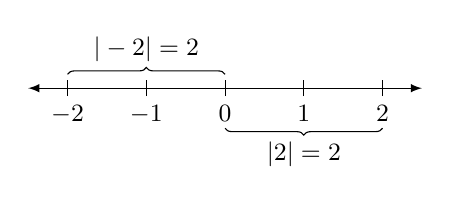
\begin{tikzpicture}
	\draw [<->, > = latex] (-2.5,0) -- (2.5,0);
	\foreach \x in {-2,-1,0,1,2}
	\draw (\x, -0.1) -- (\x, 0.1);
	\foreach \x in {-2,-1,0,1,2}
	\node at (\x, -0.1) [below] {\small $\x$};
	\draw[decoration={brace, raise=5pt},decorate] (-2,0) -- node[above=6pt] {\small $|-2|=2$} (0,0);
	\draw[decoration={brace, mirror, raise=0.2in},decorate] (0,0) -- node[below=0.22in] {\small $|2|=2$} (2,0);
\end{tikzpicture}
\end{center}
\end{frame}

\begin{frame}{Solving Absolute Value Equations}
When solving absolute value equations:

\[|x| = c \text{ means that } x=c \text{ or } x=-c\]
\pause

{\color{blue}\textbf{Make sure your absolute value bars are isolated on one side before separating your problem into 2 equations.}}
\end{frame}

\begin{frame}{Example 1}
Solve each.	\newline\\
(a) \quad $|2x-3| = 11$
\begin{align*}
\onslide<2->{2x-3 &= 11 & 2x-3 &= -11} \\[6pt]
\onslide<3->{2x &= 14 & 2x &=-8} \\[6pt]
\onslide<4->{x &= 7 & x &= -4}
\end{align*}
\onslide<5->{\[x =7 \text{ or } x = -4\]}
\end{frame}

\begin{frame}{Example 1}
(b) \quad $|3x-1| = 5$
\begin{align*}
\onslide<2->{3x-1 &= 5 & 3x-1 &= -5} \\[6pt]
\onslide<3->{3x &= 6 & 3x &=-4} \\[6pt]
\onslide<4->{x &= 2 & x &= -\frac{4}{3}}
\end{align*}
\onslide<5->{\[x =2 \text{ or } x = -\frac{4}{3}\]}
\end{frame}

\begin{frame}{Example 1}
(c) \quad $|x+1| = -2$
\begin{align*}
\onslide<2->{x+1 &= -2 & x+1 &=2} \\[6pt]
\onslide<3->{x&= -3 & x &= 1} 
\end{align*}
\onslide<4->{No solution $(\varnothing)$}
\end{frame}

\begin{frame}{Example 1}
(d) \quad $|-x+2|-4 = 10$
\begin{align*}
\onslide<2->{|-x+2| &= 14 &\text{add 4}}
\end{align*}
\begin{align*}
\onslide<3->{-x+2 &= 14 & -x+2 &= -14} \\[6pt]
\onslide<4->{-x &= 12 & -x &= -16} \\[6pt]
\onslide<5->{x &= -12 & x &= 16}
\end{align*}
\onslide<6->{\[x = -12 \text{ or } x = 16\]}
\end{frame}


\begin{frame}{Example 1}
(e) \quad $|3x-1| = |x+5|$
\begin{align*}
\onslide<2->{3x-1 &= x+5 & 3x-1 &= -(x+5)} \\[6pt]
\onslide<3->{3x-1 &= x+5 & 3x-1 &= -x-5} \\[6pt]
\onslide<4->{2x-1 &= 5 & 4x-1 &=-5} \\[6pt]
\onslide<5->{2x &= 6 & 4x &= -4} \\[6pt]
\onslide<6->{x &= 3 & x &= -1}
\end{align*}
\onslide<7->{\[x=3 \text{ or } x=-1\]}
\end{frame}


\section{Solve and graph absolute value inequalities}

\begin{frame}{Absolute Value Inequalities: $<$ and $\leq$}
Absolute value inequalities are similar to absolute value equations.	\newline\\	\pause
For $|x| < 2$, we want all values of $x$ that are \alert{less than 2 units from 0} on a number line:	\newline\\	\pause
\begin{center}
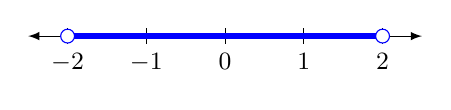
\begin{tikzpicture}
	\draw [<->, > = latex] (-2.5,0) -- (2.5,0);
	\foreach \x in {-2,-1,0,1,2}
	\draw (\x, -0.1) -- (\x, 0.1);
	\foreach \x in {-2,-1,0,1,2}
	\node at (\x, -0.1) [below] {\small $\x$};
	\draw (-2,0) [color = blue!120, fill=white] circle (2.5pt);
	\draw (2,0) [color = blue!120, fill=white] circle (2.5pt);
	\draw [line width = 2, color = blue!120] (-1.92,0) -- (1.92,0);
\end{tikzpicture}
\end{center}
\pause
\[|x| < 2 \text{ means } -2 < x < 2\]
\end{frame}

\begin{frame}{Example 2}
Solve and graph each.	\newline\\
(a) \quad $|2x-2| < 5$
\begin{align*}
\onslide<2->{-5 &< 2x-2 & 2x-2 &< 5} \\[6pt]
\onslide<3->{2x-2 &>-5 & 2x-2 &< 5} \\[6pt]
\onslide<4->{2x &> -3 & 2x &< 7} \\[6pt]
\onslide<5->{x &> -\frac{3}{2} & x &< \frac{7}{2}}
\end{align*}
\begin{center}
\onslide<6->{
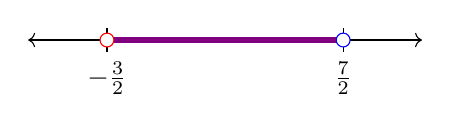
\begin{tikzpicture}
\draw[<->] (-2.5,0) -- (2.5,0);
\draw (-1.5,0.15) -- (-1.5,-0.15) node [below] {$-\frac{3}{2}$};
\draw (1.5,0.15) -- (1.5,-0.15) node [below] {$\frac{7}{2}$};
\draw[violet, line width=2] (-1.5,0) -- (1.5,0);
\draw[color=red,fill=white] (-1.5,0) circle [radius=2.5pt];
\draw[color=blue,fill=white] (1.5,0) circle [radius=2.5pt];
\end{tikzpicture}
}
\end{center}
\end{frame}

\begin{frame}{Alternate Solution Method for Example 2a}
(a) \quad $|2x-2| < 5$		\newline\\
\onslide<2->{Treat like an absolute value equation: $|2x-2|=5$ and then use \textbf{test values} in the \emph{original inequality}.}	\newline\\
\onslide<3->{$x = -\frac{3}{2} \text{ or } x = \frac{7}{2}$} \newline\\
\begin{center}
\onslide<4->{
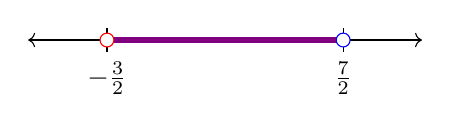
\begin{tikzpicture}
\draw[<->] (-2.5,0) -- (2.5,0);
\draw (-1.5,0.15) -- (-1.5,-0.15) node [below] {$-\frac{3}{2}$};
\draw (1.5,0.15) -- (1.5,-0.15) node [below] {$\frac{7}{2}$};
\onslide<5->{\draw[violet, line width=2] (-1.5,0) -- (1.5,0);}
\draw[color=red,fill=white] (-1.5,0) circle [radius=2.5pt];
\draw[color=blue,fill=white] (1.5,0) circle [radius=2.5pt];
\end{tikzpicture}
}
\end{center}
\end{frame}

\begin{frame}{Example 2}
(b) \quad $|x-9| \leq 2.9$
\begin{align*}
\onslide<2->{-2.9 &\leq x-9 & x-9 &\leq2.9} \\[6pt]
\onslide<3->{x-9 &\geq -2.9 & x-9 &\leq2.9} \\[6pt]
\onslide<4->{x &\geq 6.1 & x &\leq 11.9}
\end{align*}
\begin{center}
\onslide<5->{
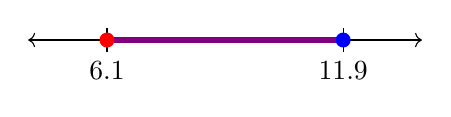
\begin{tikzpicture}
\draw[<->] (-2.5,0) -- (2.5,0);
\draw (-1.5,0.15) -- (-1.5,-0.15) node [below] {$6.1$};
\draw (1.5,0.15) -- (1.5,-0.15) node [below] {$11.9$};
\draw[violet, line width=2] (-1.5,0) -- (1.5,0);
\draw[color=red,fill=red] (-1.5,0) circle [radius=2.5pt];
\draw[color=blue,fill=blue] (1.5,0) circle [radius=2.5pt];
\end{tikzpicture}
}
\end{center}
\end{frame}

\begin{frame}{Example 2}
(c) \quad $|x+2| \leq -1$	\newline\\	\pause

No solution, $\varnothing$, since $|x+2|$ is guaranteed to always be negative.
\end{frame}

\begin{frame}{Alternate Approach to Example 2c}
(c) \quad $|x+2| \leq -1$	\qquad Treat as $|x+2|=-1$
\begin{align*}
\onslide<2->{x+2 &= -1 & x+2 &= 1} \\[6pt]
\onslide<3->{x &= -3 & x &= -1}
\end{align*}
\begin{center}
\onslide<4->{
	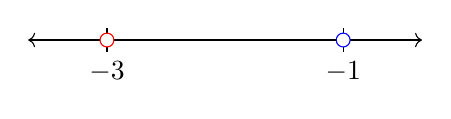
\begin{tikzpicture}
	\draw[<->] (-2.5,0) -- (2.5,0);
	\draw (-1.5,0.15) -- (-1.5,-0.15) node [below] {$-3$};
	\draw (1.5,0.15) -- (1.5,-0.15) node [below] {$-1$};
	\draw [color=red,fill=white] (-1.5,0) circle [radius = 2.5pt];
	\draw [color=blue,fill=white] (1.5,0) circle [radius = 2.5pt];
	\end{tikzpicture}
}
\end{center}
\onslide<5->{No test values work. \quad} \onslide<6->{$\varnothing$}
\end{frame}

\begin{frame}{Absolute Value Inequalities: $>$ and $\geq$}
For $|x| > 2$, we want all the values of $x$ that are \alert{greater than 2 units from 0} on a number line.	\newline\\	\pause
\begin{center}
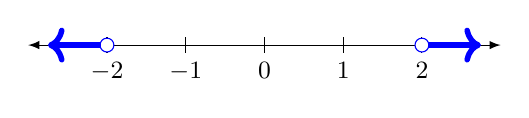
\begin{tikzpicture}
	\draw [<->, > = latex] (-3,0) -- (3,0);
	\foreach \x in {-2,-1,0,1,2}
	\draw (\x, -0.1) -- (\x, 0.1);
	\foreach \x in {-2,-1,0,1,2}
	\node at (\x, -0.1) [below] {\small $\x$};
	\draw (-2,0) [color = blue!120, fill=white] circle (2.5pt);
	\draw (2,0) [color = blue!120, fill=white] circle (2.5pt);
	\draw [->, line width = 2, color = blue!120] (-2.08,0) -- (-2.75,0);
	\draw [->, line width = 2, color = blue!120] (2.08,0) -- (2.75,0);	
\end{tikzpicture}
\end{center}
\pause
\[|x| > 2 \text{ means that } x < -2 \text{ or } x > 2 \]
\end{frame}

\begin{frame}{Example 3}
Solve and graph each.	\newline\\
(a) \quad $|2x+3| \geq 5$
\begin{align*}
\onslide<2->{2x+3 &\leq -5 & 2x+3 &\geq 5} \\[6pt]
\onslide<3->{2x &\leq -8 & 2x &\geq 2} \\[6pt]
\onslide<4->{x &\leq -4 & x &\geq 1}
\end{align*}
\begin{center}
\onslide<5->{
	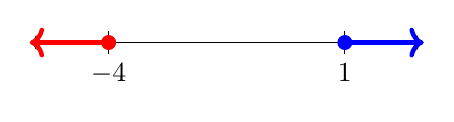
\begin{tikzpicture}
	\draw[<->] (-2.5,0) -- (2.5,0);
	\draw (-1.5,0.15) -- (-1.5,-0.15) node [below] {$-4$};
	\draw (1.5,0.15) -- (1.5,-0.15) node [below] {$1$};
	\onslide<6->{\draw [color=red,fill=red] (-1.5,0) circle [radius = 2.5pt];
							\draw[color=red,ultra thick,->] (-1.5,0) -- (-2.5,0);}
	\onslide<7->{\draw [color=blue,fill=blue] (1.5,0) circle [radius = 2.5pt];
							\draw[color=blue,ultra thick,->] (1.5,0) -- (2.5,0);}
	\end{tikzpicture}
}
\end{center}
\end{frame}

\begin{frame}{Alternate Solution Method for Example 3a}
(a) \quad $|2x+3| \geq5$		\newline\\
\onslide<2->{Treat like an absolute value equation: $|2x+3|=5$ and then use \textbf{test values} in the \emph{original inequality}.}	\newline\\
\onslide<3->{$x = -4 \text{ or } x = 1$} \newline\\
\begin{center}
\onslide<4->{
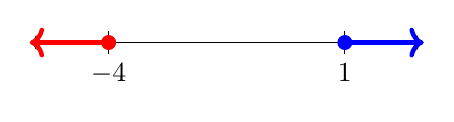
\begin{tikzpicture}
\draw[<->] (-2.5,0) -- (2.5,0);
\draw (-1.5,0.15) -- (-1.5,-0.15) node [below] {$-4$};
\draw (1.5,0.15) -- (1.5,-0.15) node [below] {$1$};
\onslide<5->{\draw[red,ultra thick, ->] (-1.5,0) -- (-2.5,0);}
\onslide<6->{\draw[blue,ultra thick, ->] (1.5,0) -- (2.5,0);}
\draw[color=red,fill=red] (-1.5,0) circle [radius=2.5pt];
\draw[color=blue,fill=blue] (1.5,0) circle [radius=2.5pt];
\end{tikzpicture}
}
\end{center}
\end{frame}

\begin{frame}{Example 3}
(b) \quad $|2x-5| > 3$
\begin{align*}
\onslide<2->{2x-5 &< -3 & 2x-5 &> 3} \\[6pt]
\onslide<3->{2x &< 2 & 2x &> 8} \\[6pt]
\onslide<4->{x &< 1 & x &> 4}
\end{align*}
\begin{center}
\onslide<5->{
	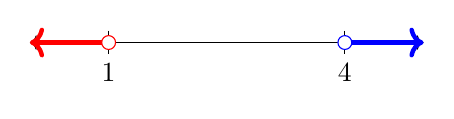
\begin{tikzpicture}
	\draw[<->] (-2.5,0) -- (2.5,0);
	\draw (-1.5,0.15) -- (-1.5,-0.15) node [below] {$1$};
	\draw (1.5,0.15) -- (1.5,-0.15) node [below] {$4$};
	\onslide<6->{\draw[color=red,ultra thick,->] (-1.5,0) -- (-2.5,0);
							\draw [color=red,fill=white] (-1.5,0) circle [radius = 2.5pt];}
	\onslide<7->{\draw[color=blue,ultra thick,->] (1.5,0) -- (2.5,0);
							\draw [color=blue,fill=white] (1.5,0) circle [radius = 2.5pt];}
	\end{tikzpicture}
					}
\end{center}
\end{frame}

\begin{frame}{Example 3}
(c) \quad $|2x+2| > -2$	\newline\\	\pause

All real numbers, $\mathbb{R}$, since $|2x+2|$ is guaranteed to always be greater than a negative number.
\end{frame}

\begin{frame}{Alternate Approach to Example 3c}
(c) \quad $|2x+2| > -2$	\qquad Treat as $|2x+2|=-2$
\begin{align*}
\onslide<2->{2x+2 &= -2 & 2x+2 &= 2} \\[6pt]
\onslide<3->{2x &= -4 & 2x &=0}	\\[6pt]
\onslide<4->{x &= -2 & x &= 0}
\end{align*}
\begin{center}
\onslide<5->{
	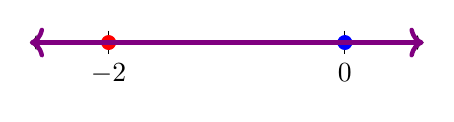
\begin{tikzpicture}
	\draw[<->] (-2.5,0) -- (2.5,0);
	\draw (-1.5,0.15) -- (-1.5,-0.15) node [below] {$-2$};
	\draw (1.5,0.15) -- (1.5,-0.15) node [below] {$0$};
	\onslide<6->{\draw [color=red,fill=red] (-1.5,0) circle [radius = 2.5pt];}
	\onslide<7->{\draw [color=blue,fill=blue] (1.5,0) circle [radius = 2.5pt];}
	\onslide<8->{\draw[<->,ultra thick, violet] (-2.5,0) -- (2.5,0);}
	\end{tikzpicture}
}
\end{center}
\onslide<9->{All test values work. \quad} \onslide<10->{$\mathbb{R}$}
\end{frame}

\end{document}